\documentclass[a4paper,12pt]{article}
\usepackage{fancyhdr}
\usepackage[ngerman,german]{babel}
\usepackage{german}
\usepackage[utf8]{inputenc}
\usepackage[active]{srcltx}
\usepackage{algorithm}
\usepackage[noend]{algorithmic}
\usepackage{amsmath}
\usepackage{amssymb}
\usepackage{amsthm}
\usepackage{bbm}
\usepackage{enumerate}
\usepackage{graphicx}
\usepackage{ifthen}
\usepackage{listings}
\usepackage{struktex}
\usepackage{hyperref}
\usepackage{tabularx}

\newcommand{\Fach}{Softwaretechnik I}
\newcommand{\Name}{Lukas Harsch}
\newcommand{\Matrikelnummer}{979272}
\newcommand{\Semester}{Wintersemester 2018/2019}
\newcommand{\Kapitel}{2}
\newcommand{\Titel}{Lineare Prozessmodelle}

\setlength{\parindent}{0em}
\topmargin 0cm
\oddsidemargin 0cm
\evensidemargin 0cm
\setlength{\textheight}{9.2in}
\setlength{\textwidth}{6.0in}

\hypersetup{
	pdftitle={\Fach{}: Kapitel \Kapitel{} - \Titel},
	pdfauthor={\Name},
	pdfborder={0 0 0}
}

\lstset{ %
	language=java,
	basicstyle=\footnotesize\tt,
	showtabs=false,
	tabsize=2,
	captionpos=b,
	breaklines=true,
	extendedchars=true,
	showstringspaces=false,
	flexiblecolumns=true,
}

\title{Kapitel \Kapitel}
\author{\Name{}}

\begin{document}
	\thispagestyle{fancy}
	\lhead{\sf \small \Name{}}
	\chead{\sf \small \Fach}
	\rhead{\sf \small \Semester{}}
	\rfoot{\sf \tiny Keine Gewähr auf Richtigkeit und Vollständigkeit}
	\lfoot{\sf \tiny Grafiken aus den Vorlesungsfolien\\CC BY-NC-SA }
	\begin{center}
		\LARGE \sf \textbf{Kapitel \Kapitel}\\
		\LARGE \sf \Titel
	\end{center}
	\vspace*{0.2cm}
	
	\section{Einführung}
	Die \textbf{zentrale Fragestellung} für das Prozessmodell ist, wie man zweckmä"sigerweise bei der Erstellung einer Software vorgeht.\\
	
	\textbf{Lebenszyklus}:\\
	Idee/Wunsche $\Rightarrow$ Entwicklung $\Rightarrow$ Gebrauch $\Rightarrow$ Wartung $\Rightarrow$ Ausmusterung\\
	
	\textbf{Entwicklungszyklus}:\\
	Entwurf $\Rightarrow$ Realisierung von Komponenten $\Rightarrow$ Zusammebau $\Rightarrow$ Prüfung
	
	\section{Prozess und Preozessmodelle}
	Ein \textbf{Prozess} ist eine Sequenz von Schritten, die für einen bestimmten Zweck ausgeführt werden.\\
	
	Beispiel eines Software-Entwicklungsprozess / Prozessmodell:
	\begin{center}
		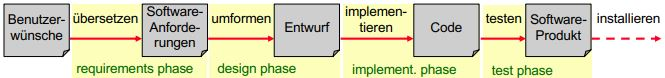
\includegraphics[width=\linewidth]{pics/se_prozess.jpg}
	\end{center}
	
	Ein \textbf{Prozessmodell} ist eine Muster-Struktur für Organisation und Durchführung eines Software-Entwicklungs-Prozesses.\\
	Bei einem Softwareentwurf geht man (noch immer gängig) mit dem \textit{Code and fix} Modell vor, also Codierung und Korrektur im Wechsel mit Ad-hoc-Tests als einzige bewusste Tätigkeiten der Software-Entwicklung. Dies ist allerdings \textbf{kein} Prozessmodell.\\
	Nach IEEE-Standart ist der Inhalt eines Prozessmodells folgenderma"sen:
	\begin{itemize}
		\item Reihenfolge des Arbeitsablaufs
		\item Durchzuführende Aktivitäten
		\item Definition der Teilprodukte
		\item Verantwortlichkeiten, Rollenverteilung und Kompetenzen
		\item Notationen, Vorgehensweisen und Werkzeuge
		\item Struktur und Merkmale der Dokumente
		\item Prüf- und Fertigstellungskriterien
	\end{itemize}
	\section{Lineare Vorgehensweisen}
	
	\subsection*{Aktivitäten-orientierte Prozessmodelle - Wasserfallmodell}
	Das Wasserfallmodell ist ein streng sequentielles "`Einbahnstra"senmodell"' und ist \textbf{Aktivitätenorientiert}, statt nach Zielen oder Ergebnissen. 
	\begin{center}
		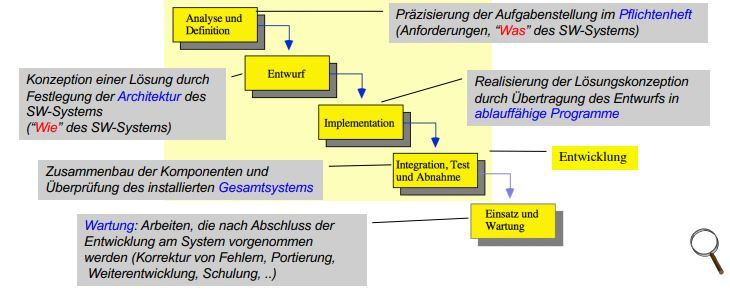
\includegraphics[width=\linewidth]{pics/wasserfallmodell.jpg}
	\end{center}
\begin{center}
	\begin{tabularx}{13cm}{X|X}
		\hline 
		Vorteile & Nachteile\\ \hline \hline
		Erstellung der Software in kleinen, überschaubaren, wohldefinierten Schritten & Idealvorstellung, die nicht der Realität entspricht \\ \hline
		Projektüberwachung und Fortschrittskontrolle an festen Messpunkten & SW-Entwicklung verläuft meist nicht linear, Prüfung am Ende zu spät 
	\end{tabularx}
\end{center}

	\subsection*{Ergebnis-orientierte Prozessmodelle - Phasenmodell}
	Beim Phasenmodell wird der Entwicklungsprozess in Abschnitte ("`Phasen"') gegliedert mit definierten Meilensteinen, welche durch inhaltliche Kriterien und nicht durch Zeitpunkte definiert sind.\\
	Eine Phase ist hierbei ein Intervall zwischen zwei Meilensteinen. Phasen sind charakterisiert durch erzielte Ergebnisse, und nicht durch Aktivitäten (wesentlicher Unterschied zum Wasserfallmodell).
	\begin{center}
		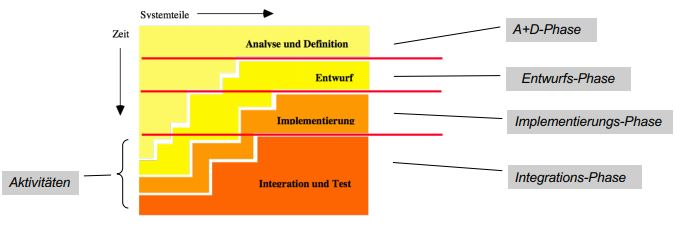
\includegraphics[width=\linewidth]{pics/phasenmodell.jpg}
	\end{center}
	Hierbei werden die Phasen sequentiell durchlaufen, wobei eine Rückkehr zu einer früheren Phase nicht vogesehen ist. Die Phasenbezeichnung gibt jeweils nur die Haupttätigkeit an.\\
	
	\textbf{Vorteile}:\\
	Klar organisierter Ablauf (wie beim Wasserfallmodell) und eine relativ einfache Projektführung (anhand von Meilensteinen).
	\subsection*{V-Modell}
	Grundidee: Beim V-Modell werden das Phasenmodell und Qualitätssicherung integriert.
	\begin{center}
		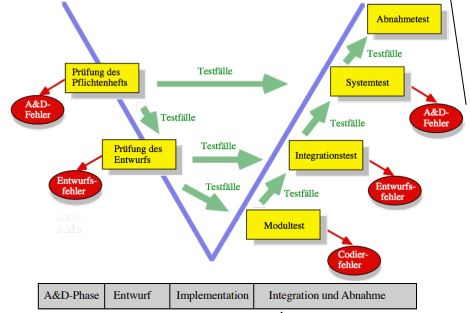
\includegraphics[width=\linewidth]{pics/vmodell.jpg}
	\end{center}
	Aufgebaut ist das V-Modell folgenderma"sen:
	\begin{itemize}
		\item Von links nach rechts erstreckt sich die Zeitachse
		\item Von oben nach unten erstreckt sich der Grad der Detaillierung
		\item Die einzelnen Phasen sind unterhalb des "`V"' aufgelistet.
		\item In der Spitze erfolgt die Implementierung, die anschlie"send auf der rechten Seite gegen die entsprechenden Spezifikationen der linken Seite getestet wird
	\end{itemize}
	Die Wesentlichen Erkenntnisse dieses Modells belaufen sich auf die verschiedenen Abstraktionsebenen des Entwicklungsprozesses, und, dass Fehler im Allgemeinen nur auf der Ebene gefunden werden, auf der sie gemacht wurde.
	
	\subsubsection*{V-Modell 97}
	Das V-Modell 97 ist eine Weiterentwicklung der Grundidee und ist nicht nur für Software, sondern auch für software-gestützte Systeme. Weitere Weiterentwicklungen:
	\begin{itemize}
		\item Verschiedene Aspekte der Standardisierung
		\item Neben Entwicklung und Qualitätssicherung (QS) auch weitere Submodelle mit definierten Zusammenhänge zwischen den Submodellen.
		\item verschiedene Abstraktionsebenen
	\end{itemize}
	Au"serdem werden \textit{Aktivitäten}, \textit{Produkte} und \textit{Zustände} des Entwicklungsprozesses festgelegt. \\
	
	\textbf{Standardisierung}:\\
	Ziel der Standardisierung ist die bessere Planbarkeit von IT-Projekten sowie die Verbesserung der Qualität und Kommunikation zwischen Auftraggeber und -nehmer.\\
	
	Beim V-Modell 97 gibt es 4 Submodelle:
	\begin{itemize}
		\item Systemerstellung (SE)
		\item Projektmanagement (PM)
		\item Qualitätssicherung (QS)
		\item Konfigurationsmanagement (KM)
	\end{itemize}
	Für jedes dieser Submodelle gibt es damit 3 Aspekte:
	\begin{itemize}
		\item Vorgehensweise: \textbf{Was} ist zu tun?
		\item Methoden: \textbf{Wie} ist etwas zu tun?
		\item Werkzeuganforderungen: \textbf{Womit} ist etwas zu tun?
	\end{itemize}
	\begin{center}
		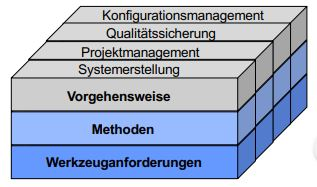
\includegraphics[scale=1.5]{pics/vmodell97.jpg}
	\end{center}
	\subsubsection*{V-Modell XT}
	Das V-Modell XT ist ein Produktzentrierter Ansatz ("`Integriertes Produktmodell"') und wird gegliedert in
	\begin{itemize}
		\item \textbf{Produkte}: stehen im Mittelpunkt, haben definierte Abhängigkeiten und sind (Zwischen-)Ergebnisse eines Projekts
		\item \textbf{Aktivitäten}: dienen dazu, um Produkte zu erzeugen oder zu bearbeiten
		\item \textbf{Rollen}: beschreiben zusammengehörige Aufgaben, Verantwortlichkeit und benötigte Fähigkeiten
	\end{itemize}
	Submodelle, Abstraktionsebenen und Erzeugnisstruktur im Wesentlichen wie bei V-Modell 97.\\
	
	\textbf{Unterschiede von V-Modell XT zu V-Modell 97}:
	\begin{itemize}
		\item Legt Rahmenvorgaben fest und bietet dadurch grö"sere \textit{Flexibilität} (bzgl. konkreter Vorgehensweise), zum Beispiel
		\begin{itemize}
			\item Inkrementell
			\item Komponentenbasiert
			\item Agil
		\end{itemize}
		\item Legt für jedes Produkt eindeutig \textit{Rollen/Verantwortlichkeiten} fest
		\item Unterscheidet \textit{verschiedene Projekttypen}
		\item Au"serdem ist das Problem- und "Anderungsmanagement ein separates Submodell
	\end{itemize}
	\begin{center}
		\begin{tabularx}{13cm}{X|X}
			\hline 
			Vorteile & Nachteile\\ \hline \hline
			Standardisierte Abwicklung von Systemerstellungsprojekten & Ohne geeignete Werkzeugunterstützung nicht handhabbar (entsprechendes Werkzeug gibt es) \\ \hline
			Integrierte Darstellung durch SE, QS, PM und KM & Gefahr von "`Software-Bürokratie"' für kleine und mittlere Systeme \\ \hline
			Generisches Vorgehensmodell mit definierten Möglichkeiten zur Anpassung $\Rightarrow$ tailoring & \\ \hline
			Gut geeignet für gro"se Systeme mit langer Lebensdauer und Outsourcing & 
			
		\end{tabularx}
	\end{center}
	\newpage
	\subsection*{Spiralmodell}
	Das Spiralmodell nach Boehm ist ein \textit{Generisches Modell} mit Vorteilen für das Projektmanagement.\\
	In jedem Entwicklungsschritt (= eine Spiralwindung) gibt es folgende Phasen:
	\begin{itemize}
		\item Zielbestimmung, Alternativen
		\item Evaluation der Alternativen, Erkennung und Reduktion vo Risiken
		\item Entwicklung und Validation des jeweiligen Zwischenproduktes
		\item Review des Zwischenproduktes und Planung der Folgeaktivität
	\end{itemize}
	\begin{center}
		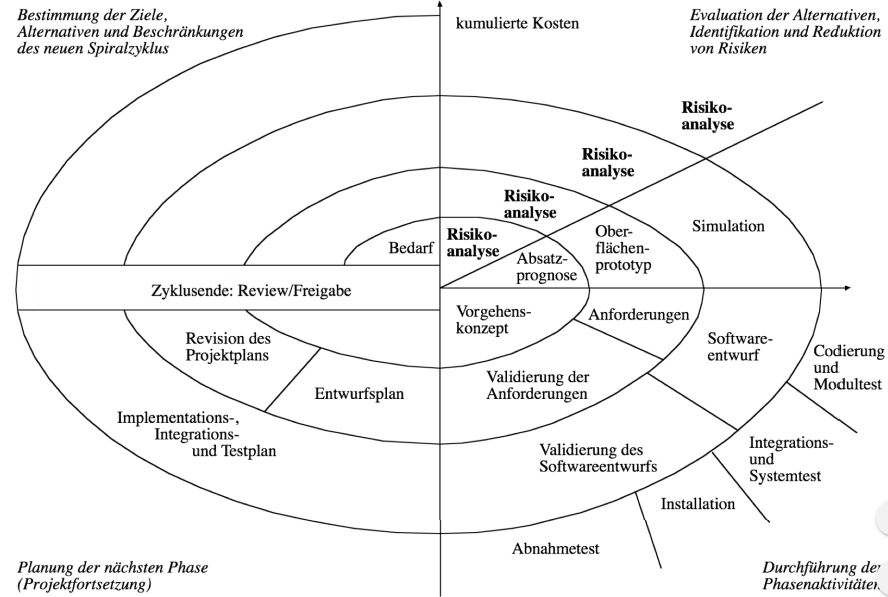
\includegraphics[width=\linewidth]{pics/spiralmodell.jpg}
	\end{center}
	\begin{center}
		\begin{tabularx}{13cm}{X|X}
			\hline 
			Vorteile & Nachteile\\ \hline \hline
			Fehler und ungeeignete Alternativen werden frühzeitig eliminiert & Hoher Managementaufwand \\ \hline
			Flexibler Prozessablauf & 
		\end{tabularx}
	\end{center}
\end{document}